\documentclass[12pt]{article}
\usepackage{graphicx}
\usepackage {color}
\usepackage{pdfpages}
\usepackage{float}
\usepackage{changebar}
\usepackage{enumitem,amssymb}
\renewcommand{\familydefault}{\sfdefault}
\usepackage[margin=1.2in]{geometry}
\usepackage{graphicx}
\usepackage{wrapfig}
\usepackage[super]{cite}
\usepackage{subcaption}
\usepackage[table]{xcolor}
\usepackage{amsmath}
\usepackage[sort, numbers]{natbib}
\usepackage{multirow}
\usepackage{tabularx}
\usepackage{siunitx}
\usepackage{matlab-prettifier}
\usepackage{wrapfig,lipsum,booktabs}
%%%%%%%%%%%%Defining the margins %%%%%%%%%%%%%%%%%%%%%
\textheight 9.in
\textwidth 6.5in
\topmargin -.5in
\oddsidemargin 0in
\setlength{\parskip}{\smallskipamount}

%%%%%%%%%%%%%%Specific Commands %%%%%%%%%%%%%%%%%%
\newcommand{\eg}{{\em e.g.,}}
\newcommand{\ie}{{\em i.e.,}}
\newcommand{\etc}{{\em etc.,}}
\newcommand{\etal}{{\em et al.}}
\newcommand{\degrees}{{$^{\circ}$}}
\newcommand{\fig}[1]{\textbf{Figure #1}}

%%%%%%%%%%%%%%%%%%%%%%%%%%%% Setting to control figure placement
% These determine the rules used to place floating objects like figures 
% They are only guides, but read the manual to see the effect of each.
\renewcommand{\topfraction}{.9}
\renewcommand{\bottomfraction}{.9}
\renewcommand{\textfraction}{.1}
\renewcommand{\familydefault}{\sfdefault} %setting the san serif font

%%%%%%%%%%%%%%%%%%%%%%%% Line spacing
% Use the following command for ``double'' spacing
%\setlength{\baselineskip}{1.2\baselineskip}
% and this one for an acceptable NIH spacing of 6lpi based on 11pt
%\setlength{\baselineskip}{.9\baselineskip}
% The baselineskip does not appear to work when we include a maketitle
% command in the main file.  Something there must set the line spacing
% If we use this next command, then things seem to work.
\renewcommand{\baselinestretch}{.9}

\setcounter{secnumdepth}{0} %make no numbers but have a table of contents


\begin{document}

\title{HW 4: Medical Imaging Systems}
\author{Jake Bergquist, u6010393 }
\maketitle

\section{Q1}
\noindent\textbf{a: } 
Attached is the drawn sinogram for (a). All of the profiles are either semicircular or semi oval with a smooth transition between the different angles.

\noindent\textbf{b: } 
Attached is the drawn sinogram for (b). All profiles have either a semicircle, or two, or some overlap of two. The 0 degree projection has double the peak intensity of any of the projections where the two semicircles do not overlap. One of the circles is closer to the center than the other leading to the kind of mirroring effect seen in the sinogram profile.

\noindent\textbf{c: }
Attached is the sinogram for (c). All profiles are either trapezoids, rectangles or triangles. Assuming a uniform diffusion coefficient the max intensity of the 45 degree projections (ones that cross the diagonal of the square perfectly) is $\sqrt{2}$ larger than the max intensity of the 0 or 90 degree projections (the ones that are parallel to the sides of the square). Here max intensity meaning the maximum projection on the sinogram which corresponds to the maximal attenuation of the X ray beam through the sample.

\section{Q2}
\noindent\textbf{a: } 
The predicted object for part (a) is attached. The pattern of a small rectangle profile with high intensity at 0 and a large rectangular profile with less intensity at 90 or -90 suggests an object like a rectangle that is wider on the 90 degree projections than the 0 degree. Additionally there is a triagle profile at some angle less than 45 degrees which is the angle at which the projection would pass directly along the diagonal of the rectangle.

\noindent\textbf{b: }
The drawn object prediction is attached. For this one there seems to be a circle of lower attenuation coefficient centered at the origin . The remaining profile looks like an ofset oval like shape along the y axis as shown.

\section{Q3}
\noindent\textbf{a: }
Below is my function. Figure~\ref{basic} shows the results of 0, 30 and 45 degree projections of a rectangualr profile.

\begin{figure}[H]
	
	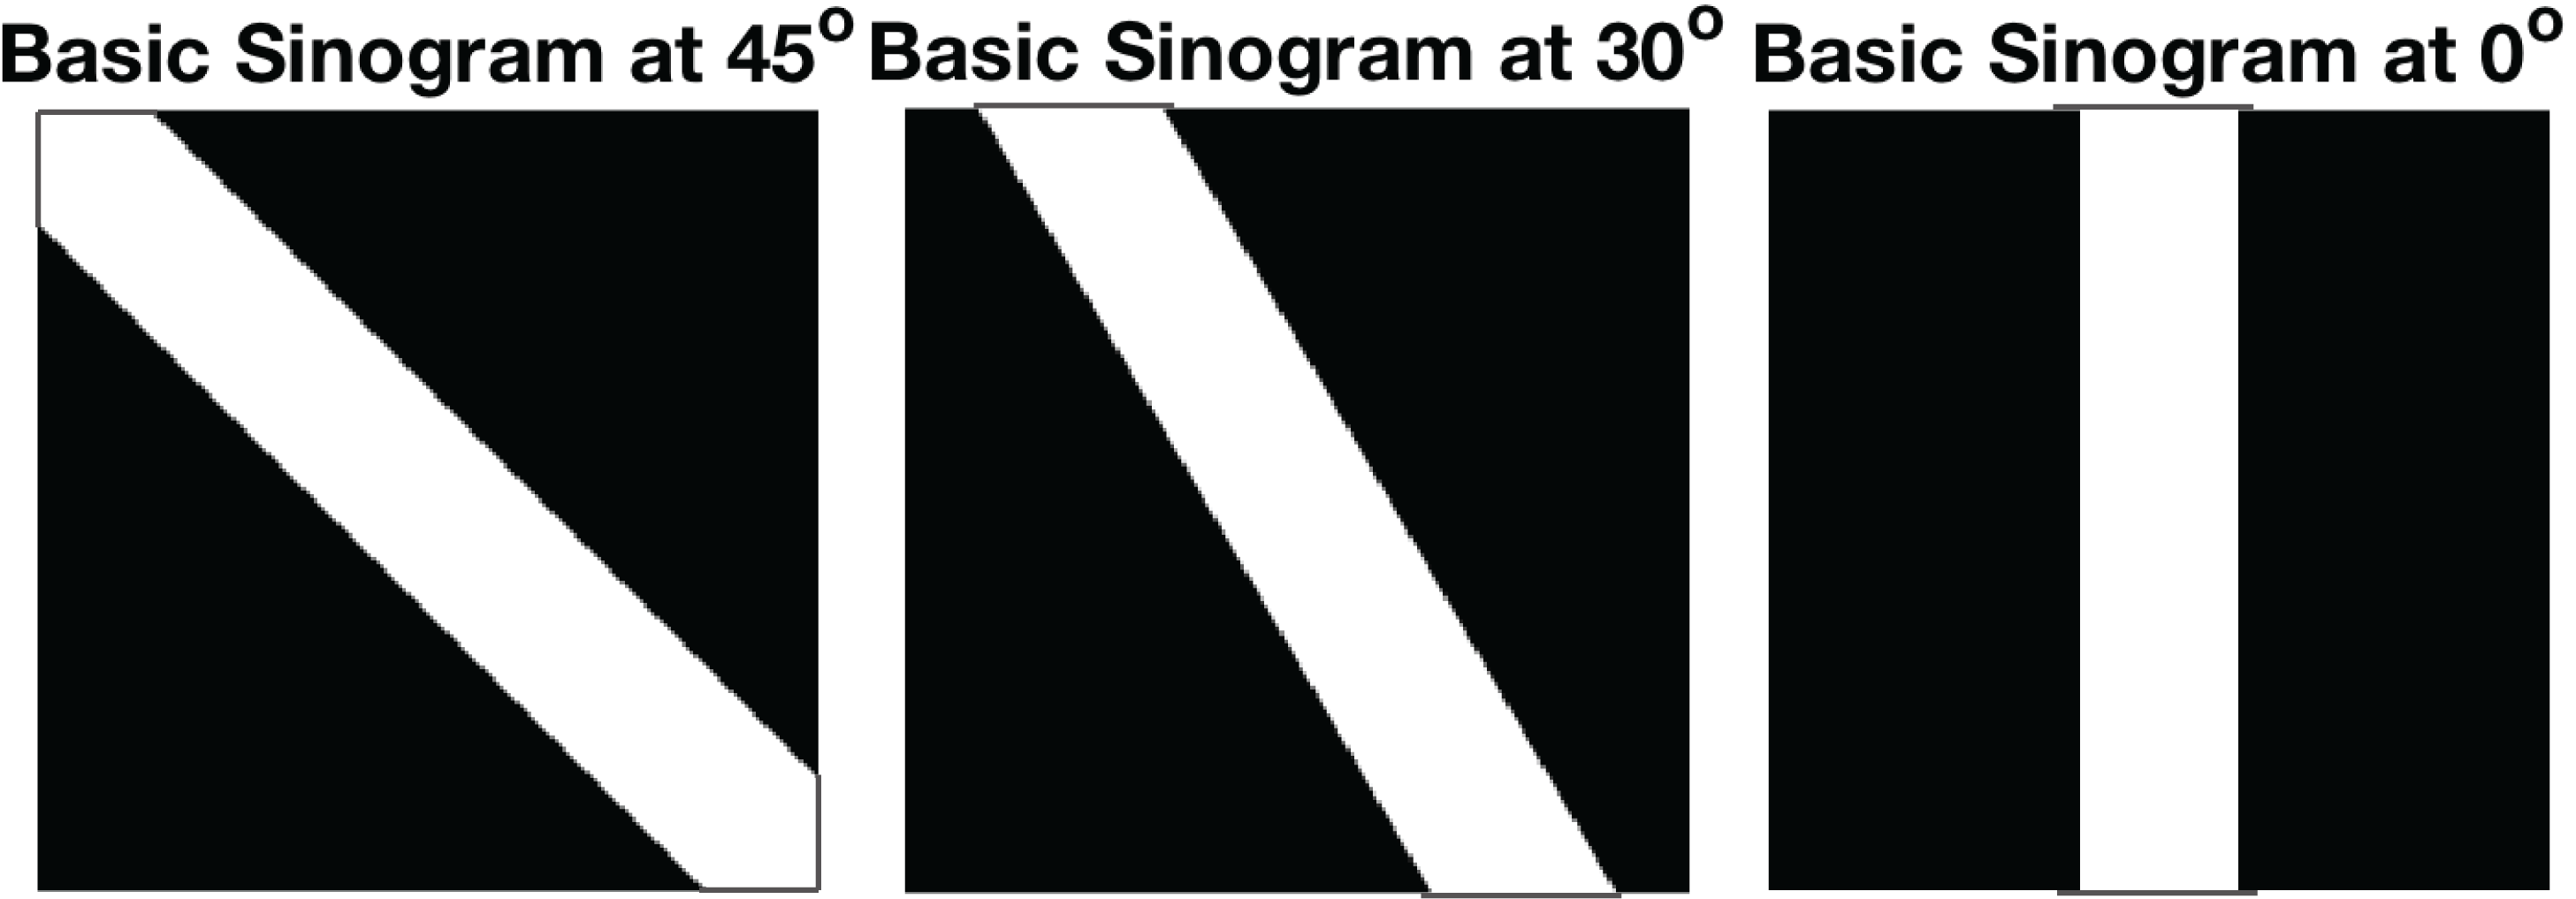
\includegraphics[width=\textwidth]{basicone.png}
	\caption{Basic sinogram projections for 0, 30, and 45 degrees for a rectangular profile.}
	\label{basic}
\end{figure}
\begin{lstlisting}[style=Matlab-editor]
function [Btheta] = BackPropSinogram(Rtheta,theta,interp)
%Input: Rtheta: the inogram projection at theta
%       Theta: the angle of the current projection
%       Interp: The interpolation method fromt eh fit function
%               Default: 'linearinterp'
%Assume image center is at the origin
%Assume Rtheta has an odd number of measurements

if ~exist(interp)
	interp = 'linearinter';
end


imageLim = floor(length(Rtheta)/2);
[X,Y] = meshgrid([-imageLim:imageLim],[imageLim:-1:-imageLim]);
RotCoords1 = Y.*sin(theta) + X.*cos(theta);
RotCoords2 = Y.*sin(pi/2-theta) + X.*cos(pi/2-theta);
Val = repmat(Rtheta,1,size(X,2));
sf = fit([X(:),Y(:)],Val(:),interp);
Btheta = sf(RotCoords2,RotCoords1);
Btheta(isnan(Btheta)) = 0;

%Below is the minimum line version of above
%I chose to go with what is above because it is easier to read
%Both version produce the same output
%    [X,Y] = meshgrid([-floor(length(Rtheta)/2):floor(length(Rtheta)/2)],[floor(length(Rtheta)/2):-1:-floor(length(Rtheta)/2)]);
%    sf = fit([X(:),Y(:)],reshape(repmat(Rtheta,1,size(X,2)),[length(Rtheta)*size(X,2),1]),interp);
%    Btheta = sf(Y.*sin(pi/2-theta) + X.*cos(pi/2-theta),Y.*sin(theta) + X.*cos(theta));
%    Btheta(isnan(Btheta)) = 0;
end
\end{lstlisting}

\noindent\textbf{b: }
Figure~\ref{sino} shows the provided sinogram with 0, 90, and 180 degrees marked.
\begin{figure}[H]
	
	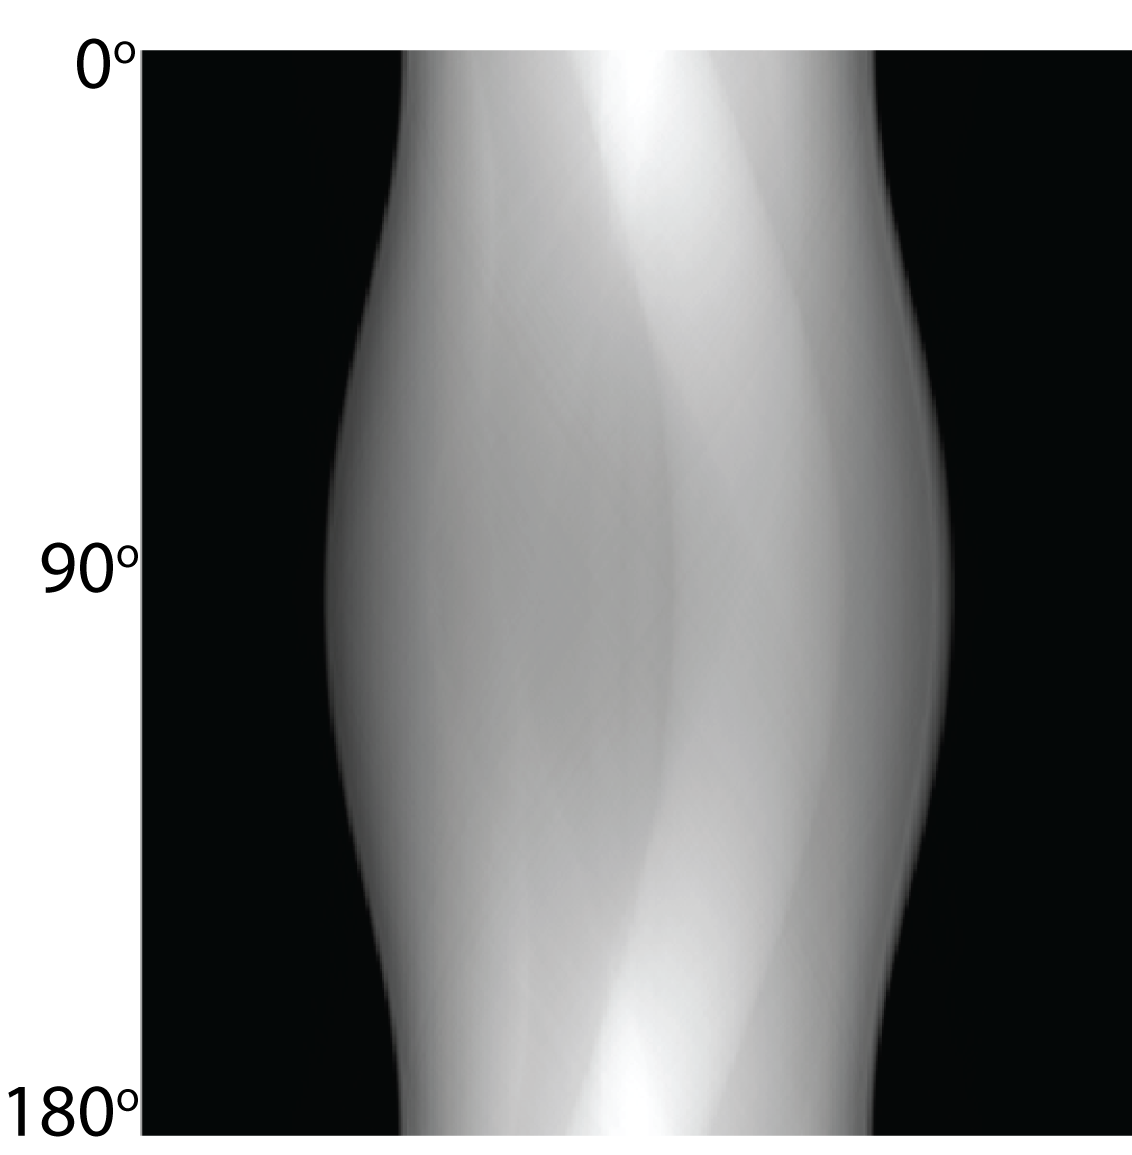
\includegraphics[width=\textwidth]{sinogram.png}
	\caption{Provided sinogram with 0, 90, and 180 degrees marked.}
	\label{sino}
\end{figure}

\noindent\textbf{c\&d: }
In Figure~\ref{direct} we see the results of backprojection. This is a very blurred image but we can barely make out that there seems to be some circular shape with perhaps another circle of different consistency within it.

\section{Q4}

\section{Q5}






\begin{lstlisting}[style=Matlab-editor]
%%


\end{lstlisting}

\end{document}



\begin{figure}[H]
	\centering
	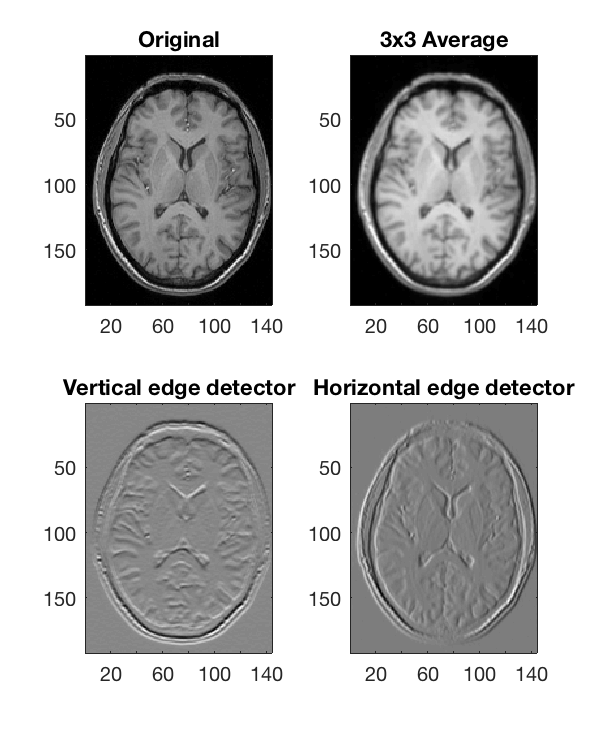
\includegraphics[width=\textwidth]{Figures/convs.png}
	\caption{}
	\label{Fig:conv}
\end{figure}

\begin{lstlisting}[style=Matlab-editor]

\end{lstlisting}




